\documentclass[aspectratio=169,11pt]{beamer}

% ---------------------------------------------------------
% TP1 - Visualização Geométrica, Rasterização e Recorte de Árvores CCO
% BCC327 - Computação Gráfica - UFOP - 2026.2
% ---------------------------------------------------------

% --- PACOTES PRINCIPAIS ---
\usepackage[utf8]{inputenc}
\usepackage[T1]{fontenc}
\usepackage{amsmath, amssymb, amsfonts}
\usepackage{booktabs}
\usepackage{tabularx}
\usepackage{graphicx}
\usepackage{xcolor}
\usepackage{hyperref}
\usepackage{listings}
\usepackage{tikz}
\usetikzlibrary{positioning}

\graphicspath{{figures/}}
\renewcommand{\figurename}{Figura}
\renewcommand{\tablename}{Tabela}

% --- CORES INSTITUCIONAIS / ESTILO ---
\definecolor{ufopred}{RGB}{140,29,36}
\definecolor{deepnavy}{RGB}{20,35,60}
\definecolor{lightgray}{RGB}{245,247,250}
\definecolor{darkslate}{RGB}{30,40,50}
\definecolor{softblue}{RGB}{230,238,247}

% --- TEMA BEAMER ---
\usetheme{Madrid}
\usecolortheme{default}
\setbeamertemplate{navigation symbols}{}
\setbeamercolor{structure}{fg=ufopred}
\setbeamercolor{frametitle}{fg=white,bg=ufopred}
\setbeamercolor{title}{fg=white,bg=ufopred}
\setbeamercolor{block title}{fg=white,bg=deepnavy}
\setbeamercolor{block body}{fg=black,bg=lightgray}
\setbeamercolor{alerted text}{fg=ufopred}

% --- RODAPE PERSONALIZADO ---
\setbeamertemplate{footline}{%
  \leavevmode%
  \hbox{%
    \begin{beamercolorbox}[wd=.72\paperwidth,ht=2.6ex,dp=1.1ex,leftskip=1.5ex]{author in head/foot}%
      \textcolor{darkslate}{\insertshorttitle}
    \end{beamercolorbox}%
    \begin{beamercolorbox}[wd=.28\paperwidth,ht=2.6ex,dp=1.1ex,rightskip=1.5ex plus1fil]{date in head/foot}%
      \hfill \textcolor{darkslate}{\insertframenumber/\inserttotalframenumber}
    \end{beamercolorbox}%
  }%
}

% --- CONFIGURACAO DE CODIGO ---
\lstset{
  basicstyle=\ttfamily\small,
  keywordstyle=\color{ufopred}\bfseries,
  commentstyle=\color{darkslate},
  stringstyle=\color{deepnavy},
  showstringspaces=false,
  frame=single,
  rulecolor=\color{lightgray},
  breaklines=true
}

% --- COMANDOS UTEIS ---
\newcommand{\checkitem}{\textcolor{ufopred}{$\blacktriangleright$}}
% imagem com legenda curta embaixo
\newcommand{\fig}[3]{%
  \begin{minipage}[t]{#1\textwidth}\centering
    \includegraphics[width=\linewidth]{#2}\\[-0.05cm]
    {\scriptsize #3}
  \end{minipage}}

% ---------------------------------------------------------
% DADOS DA APRESENTACAO
% ---------------------------------------------------------
\title[TP1 CCO | Brenda Gabrielle Alves Nascimento (24.1.4011)]{Visualização Geométrica, Rasterização e Recorte de Árvores Arteriais CCO}
\subtitle{BCC327 -- Computação Gráfica | Trabalho Prático 1}
\author{Brenda Gabrielle Alves Nascimento\\{\small Matrícula 24.1.4011}}
\institute[UFOP]{Departamento de Computação (DECOM)\\Universidade Federal de Ouro Preto (UFOP)}
\date{2026.2 | Prof. Dr. Rafael Alves Bonfim de Queiroz}

% ---------------------------------------------------------
\begin{document}

\begin{frame}
  \titlepage
\end{frame}

\begin{frame}{Roteiro da Apresentação}
\tableofcontents
\end{frame}

% =========================================================
\section{Contexto e Objetivos}
% =========================================================

\begin{frame}{Contexto: árvores arteriais CCO}
\begin{columns}[c]
\column{0.42\textwidth}
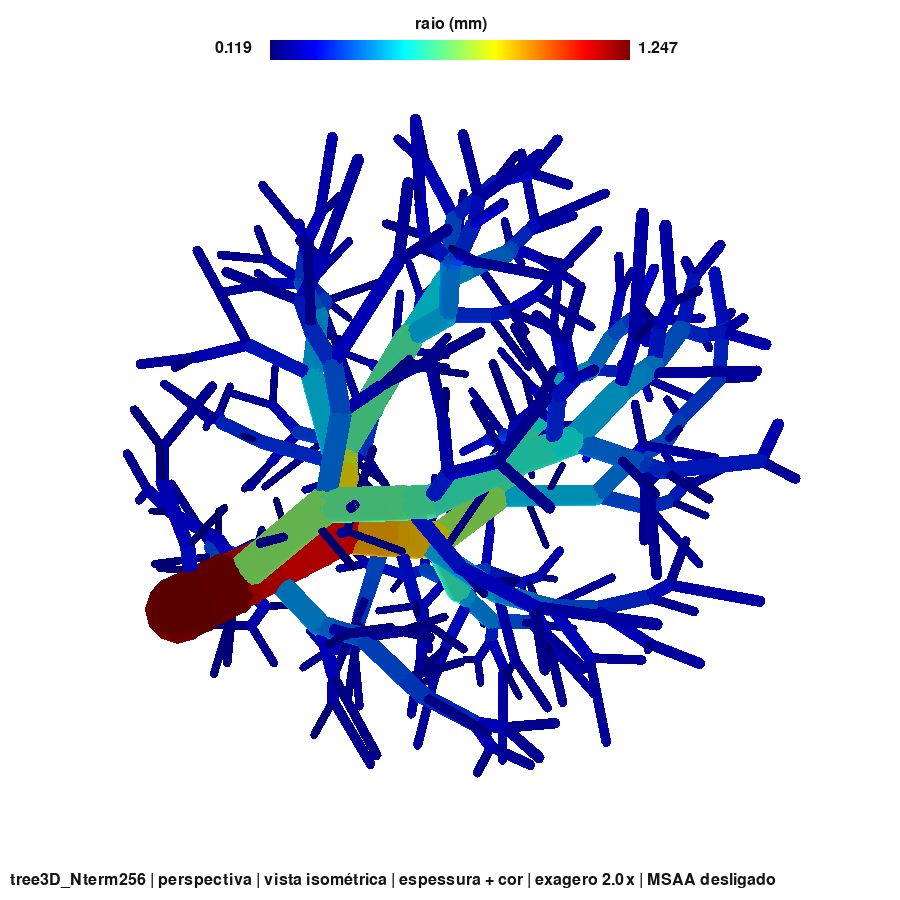
\includegraphics[width=\linewidth]{m1_tubos_3d}

\column{0.55\textwidth}
\begin{block}{Arquivo VTK (POLYDATA)}
\small
\texttt{POINTS} \quad coordenadas $(x, y, z)$\\
\texttt{LINES} \quad\ \ segmentos \texttt{2 i j}\\
\texttt{CELL\_DATA} \texttt{raio} por segmento (mm)
\end{block}
\vspace{0.2cm}
\small
\begin{tabular}{lccc}
\toprule
& \textbf{Modelos} & \textbf{Pontos} & \textbf{Segmentos}\\
\midrule
2D & 6 & 16 a 512 & 15 a 511\\
3D & 6 & 32 a 1024 & 31 a 1023\\
\bottomrule
\end{tabular}

\vspace{0.15cm}
\checkitem\ sempre $\text{segmentos} = \text{pontos} - 1$: uma árvore
\end{columns}
\end{frame}

\begin{frame}{Arquitetura: dois programas, mesmos módulos}
\begin{center}
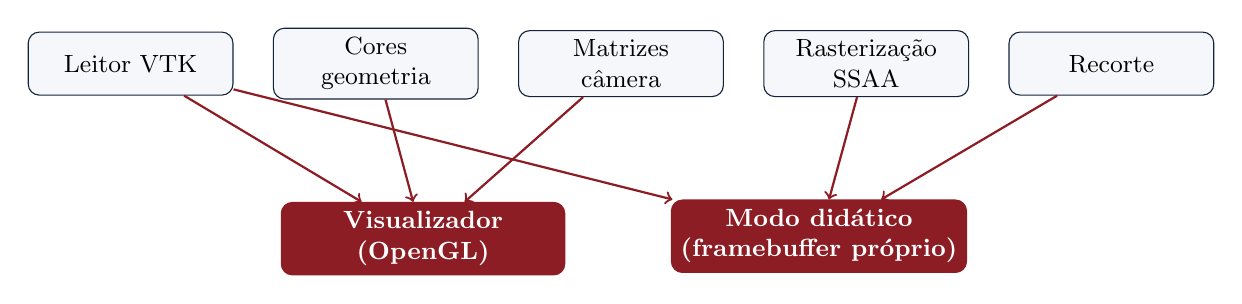
\begin{tikzpicture}[
  caixa/.style={draw=deepnavy, fill=lightgray, rounded corners, align=center,
                minimum width=2.6cm, minimum height=0.8cm, font=\small},
  prog/.style={draw=ufopred, fill=ufopred, text=white, rounded corners, align=center,
               minimum width=3.6cm, minimum height=0.9cm, font=\small\bfseries},
  seta/.style={->, thick, ufopred}]
\node[caixa] (vtk) {Leitor VTK};
\node[caixa, right=0.5cm of vtk] (cor) {Cores\\geometria};
\node[caixa, right=0.5cm of cor] (mat) {Matrizes\\câmera};
\node[caixa, right=0.5cm of mat] (ras) {Rasterização\\SSAA};
\node[caixa, right=0.5cm of ras] (rec) {Recorte};
\node[prog, below=1.3cm of cor, xshift=0.6cm] (vis) {Visualizador\\(OpenGL)};
\node[prog, below=1.3cm of ras, xshift=-0.6cm] (did) {Modo didático\\(framebuffer próprio)};
\draw[seta] (vtk) -- (vis); \draw[seta] (cor) -- (vis); \draw[seta] (mat) -- (vis);
\draw[seta] (vtk) -- (did); \draw[seta] (ras) -- (did); \draw[seta] (rec) -- (did);
\end{tikzpicture}
\end{center}
\vspace{0.3cm}
\begin{block}{Ideia central}
No modo didático, \alert{nenhum pixel vem da biblioteca}: o pygame-ce só amplia a matriz NumPy escrita pelos nossos algoritmos.
\end{block}
\end{frame}

% =========================================================
\section{Visualizador}
% =========================================================

\begin{frame}{Primitivas e atributos visuais}
\centering
\fig{0.24}{m1_linhas_jet}{linhas}\hfill
\fig{0.24}{m1_faixas_jet}{faixas + jet}\hfill
\fig{0.24}{m1_faixas_viridis}{faixas + viridis}\hfill
\fig{0.24}{m1_solido}{espessura sólida}

\vspace{0.3cm}
\small
\begin{columns}[t]
\column{0.48\textwidth}
\checkitem\ cor: $t = \dfrac{r - r_{\min}}{r_{\max} - r_{\min}}$, interpolação RGB\\
\checkitem\ jet: contraste | viridis: uniforme
\column{0.48\textwidth}
\checkitem\ faixa = 2 triângulos + discos nas pontas\\
\checkitem\ 3D: cilindros + esferas nas junções
\end{columns}
\end{frame}

\begin{frame}{Transformações geométricas}
\centering
\fig{0.24}{m2_original}{original}\hfill
\fig{0.24}{m2_translacao}{translação}\hfill
\fig{0.24}{m2_rotacao}{rotação $35^\circ$}\hfill
\fig{0.24}{m2_escala}{escala $0{,}6$}

\vspace{0.4cm}
\begin{block}{Matrizes próprias em coordenadas homogêneas}
\centering
$\mathbf{p}' = P \cdot V \cdot M \cdot \mathbf{p}$ \qquad $M = T \cdot R_x R_y R_z \cdot S \cdot N$\\[0.1cm]
{\small validadas contra \texttt{glOrtho}, \texttt{gluPerspective} e \texttt{gluLookAt}}
\end{block}
\end{frame}

\begin{frame}{Observador: quatro vistas}
\centering
\fig{0.24}{m2_vista_frontal}{frontal}\hfill
\fig{0.24}{m2_vista_lateral}{lateral}\hfill
\fig{0.24}{m2_vista_superior}{superior}\hfill
\fig{0.24}{m2_vista_isometrica}{isométrica}

\vspace{0.3cm}
\small
\begin{columns}[t]
\column{0.48\textwidth}
\textbf{Espaço do mundo}: referencial fixo da cena\\
\textbf{Espaço da câmera}: câmera na origem, olhando para $-z$
\column{0.48\textwidth}
$\mathbf{w} = \dfrac{\mathbf{e} - \mathbf{a}}{\|\mathbf{e} - \mathbf{a}\|}$, \quad
$\mathbf{u} = \mathbf{c} \times \mathbf{w}$, \quad
$\mathbf{v} = \mathbf{w} \times \mathbf{u}$
\end{columns}
\end{frame}

\begin{frame}{Projeção perspectiva $\times$ ortográfica}
\centering
\fig{0.36}{m2_perspectiva}{perspectiva: o tronco próximo fica maior}\hspace{0.6cm}
\fig{0.36}{m2_ortografica}{ortográfica: espessura não depende da distância}

\vspace{0.2cm}
\small
\checkitem\ diferença está na última linha: $(0, 0, -1, 0)$ copia a profundidade para $w$\quad
\checkitem\ caixa ortográfica com $h = d \tan(\text{fovy}/2)$
\end{frame}

% =========================================================
\section{Modo Didático}
% =========================================================

\begin{frame}{Rasterização de segmentos: Bresenham}
\begin{columns}[c]
\column{0.42\textwidth}
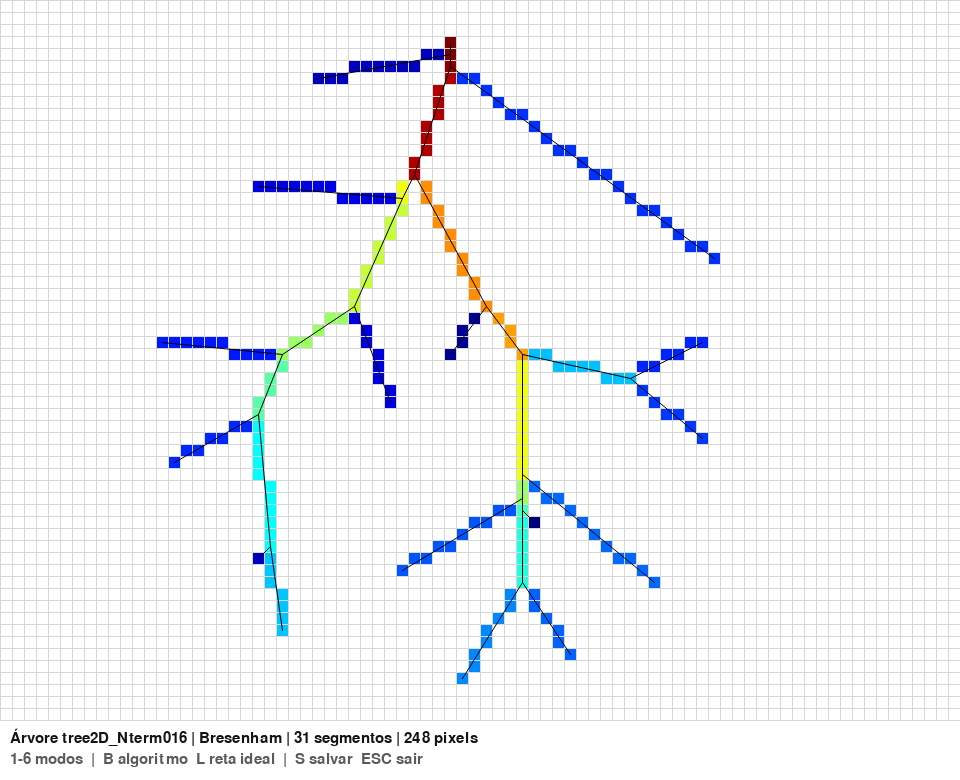
\includegraphics[width=\linewidth]{m3_arvore_bresenham}

\column{0.56\textwidth}
\small
$p_0 = 2\Delta y - \Delta x$\\[0.1cm]
$p < 0$: mantém $y$, \ $p \mathrel{+}= 2\Delta y$\\
$p \ge 0$: $y{+}{+}$, \ $p \mathrel{+}= 2\Delta y - 2\Delta x$

\vspace{0.3cm}
\scriptsize
\setlength{\tabcolsep}{3pt}
\begin{tabular}{c|ccccccccccc}
\toprule
$k$ & 0 & 1 & 2 & 3 & 4 & 5 & 6 & 7 & 8 & 9 & 10\\
$p_k$ & 6 & 2 & \alert{$-2$} & 14 & 10 & 6 & 2 & \alert{$-2$} & 14 & 10 & 6\\
$y$ & 10 & 11 & 12 & 12 & 13 & 14 & 15 & 16 & 16 & 17 & 18\\
\bottomrule
\end{tabular}

\vspace{0.2cm}
\small
\checkitem\ $(20,10)$ a $(30,18)$: só inteiros\\
\checkitem\ 20\,000 segmentos testados: erro $\le 0{,}5$ pixel
\end{columns}
\end{frame}

\begin{frame}{Preenchimento: Scanline Fill}
\centering
\fig{0.36}{m4_scanline_animacao}{varredura em andamento}\hspace{0.6cm}
\fig{0.36}{m4_scanline}{região de interesse preenchida}

\vspace{0.2cm}
\small
\begin{columns}[t]
\column{0.32\textwidth}\centering \checkitem\ tabela de arestas:\\ $(y_{\max},\ x,\ 1/m)$
\column{0.32\textwidth}\centering \checkitem\ arestas ativas ordenadas,\\ preenche aos pares
\column{0.32\textwidth}\centering \checkitem\ coerência entre linhas:\\ $x \mathrel{+}= 1/m$
\end{columns}
\end{frame}

\begin{frame}{Aliasing e antialiasing}
\centering
\fig{0.38}{m5_ssaa_leque}{sem AA $\times$ SSAA $4\times$ (16 amostras)}\hfill
\fig{0.2}{m5_msaa_off_zoom}{sem MSAA}\hfill
\fig{0.2}{m5_msaa_on_zoom}{MSAA $4\times$}

\vspace{0.25cm}
\small
\begin{columns}[t]
\column{0.48\textwidth}
\textbf{SSAA (nosso)}: grade $k\times$ maior + média dos blocos $k \times k$
\column{0.48\textwidth}
\textbf{MSAA (OpenGL)}: amostras de cobertura, cor calculada uma vez; FBO + \texttt{glBlitFramebuffer}
\end{columns}
\end{frame}

\begin{frame}{Recorte de segmentos}
\centering
\fig{0.3}{m6_recorte_antes}{antes}\hspace{0.4cm}
\fig{0.3}{m6_recorte_depois}{depois}

\vspace{0.15cm}
\scriptsize
\begin{tabular}{lll}
\toprule
& \textbf{Cohen--Sutherland} & \textbf{Liang--Barsky}\\
\midrule
Ideia & códigos de região de 4 bits & paramétrico, $t_0$ e $t_1$\\
Exemplo $(2,6)$--$(36,30)$ & 3 interseções (1 desperdiçada) & 4 razões $q/p$, 2 pontos\\
100\,000 segmentos & \multicolumn{2}{c}{resultados idênticos}\\
\bottomrule
\end{tabular}

\vspace{0.1cm}
\checkitem\ Cyrus--Beck: generaliza o Liang--Barsky para qualquer janela convexa
\end{frame}

\begin{frame}{Recorte de polígonos: Sutherland--Hodgman $\times$ Weiler--Atherton}
\centering
\fig{0.24}{m7_sh_u_depois}{S--H: 1 polígono + ponte}\hfill
\fig{0.24}{m7_wa_u_depois}{W--A: 2 polígonos}\hfill
\fig{0.24}{m7_sh_l_concavo}{S--H, janela côncava}\hfill
\fig{0.24}{m7_wa_l_concavo}{W--A, janela côncava}

\vspace{0.3cm}
\begin{block}{Weiler--Atherton (diferencial)}
\small
Percorre as duas fronteiras trocando nas interseções: aceita polígonos côncavos e devolve regiões separadas.
\end{block}
\end{frame}

% =========================================================
\section{Discussão e Conclusão}
% =========================================================

\begin{frame}{O que foi implementado pelo grupo}
\small
\begin{tabularx}{\textwidth}{X X}
\toprule
\textbf{Grupo} & \textbf{Biblioteca}\\
\midrule
Leitor VTK, mapas de cores & Janela, teclado, mouse, texto (pygame-ce)\\
Faixas 2D e tubos 3D com normais & Rasterização final dos triângulos (OpenGL)\\
Matrizes de transformação, câmera e projeção & Teste de profundidade, iluminação dos tubos\\
Bresenham, DDA, Scanline Fill & MSAA via FBO, VBOs\\
Supersampling (SSAA) & Operações vetoriais (NumPy)\\
Cohen--Sutherland, Liang--Barsky &\\
Sutherland--Hodgman, Weiler--Atherton &\\
\bottomrule
\end{tabularx}
\end{frame}

\begin{frame}{Discussão}
\begin{columns}[t]
\column{0.48\textwidth}
\begin{block}{Decisões}
\small
\checkitem\ espessura como geometria, não \texttt{glLineWidth}\\
\checkitem\ recorte em coordenadas reais, depois rasterização\\
\checkitem\ MSAA por FBO (WSL sem janela multiamostrada)
\end{block}
\column{0.48\textwidth}
\begin{block}{Limitações}
\small
\checkitem\ Nterm512 em tubos lento com renderização por software\\
\checkitem\ iluminação da API (tema do TP2)\\
\checkitem\ W--A trata degenerados por deslocamento numérico
\end{block}
\end{columns}
\end{frame}

\begin{frame}{Conclusões}
\begin{itemize}
  \item[\checkitem] 12 modelos lidos e representados por linhas, faixas e tubos
  \item[\checkitem] transformações, vistas e projeções com matrizes próprias
  \item[\checkitem] rasterização, preenchimento, antialiasing e recorte implementados e validados
  \item[\checkitem] Weiler--Atherton como diferencial
\end{itemize}
\vspace{0.3cm}
\begin{block}{Mensagem final}
Separar visualizador e modo didático permitiu mostrar cada algoritmo pixel a pixel, sem caixa-preta.
\end{block}
\end{frame}

\begin{frame}{Demonstração}
\begin{columns}[t]
\column{0.48\textwidth}
\textbf{Visualizador}
\small
\begin{itemize}
  \item[\checkitem] \texttt{E} representação, \texttt{C} cores
  \item[\checkitem] mouse: rotação e zoom
  \item[\checkitem] \texttt{1}--\texttt{4} vistas, \texttt{P} projeção
  \item[\checkitem] \texttt{M} MSAA
\end{itemize}
\column{0.48\textwidth}
\textbf{Modo didático}
\small
\begin{itemize}
  \item[\checkitem] \texttt{1}, \texttt{2} Bresenham
  \item[\checkitem] \texttt{3} + \texttt{Espaço} Scanline
  \item[\checkitem] \texttt{4} SSAA
  \item[\checkitem] \texttt{5} recorte de segmentos
  \item[\checkitem] \texttt{6} + \texttt{P}, \texttt{W}, \texttt{J} recorte de polígonos
\end{itemize}
\end{columns}
\end{frame}

\begin{frame}{Referências}
\small
\begin{thebibliography}{99}
\bibitem{schreiner1993} SCHREINER, W.; BUXBAUM, P. F. Computer-optimization of vascular trees. \textit{IEEE Transactions on Biomedical Engineering}, 1993.
\bibitem{foley} FOLEY, J. D. et al. \textit{Computer Graphics: Principles and Practice}. Addison-Wesley, 1990.
\bibitem{hearn} HEARN, D.; BAKER, M. P. \textit{Computer Graphics, C Version}. Prentice Hall, 1997.
\bibitem{bresenham} BRESENHAM, J. E. Algorithm for computer control of a digital plotter. \textit{IBM Systems Journal}, 1965.
\bibitem{liang} LIANG, Y.-D.; BARSKY, B. A. A new concept and method for line clipping. \textit{ACM TOG}, 1984.
\bibitem{sh} SUTHERLAND, I. E.; HODGMAN, G. W. Reentrant polygon clipping. \textit{CACM}, 1974.
\bibitem{wa} WEILER, K.; ATHERTON, P. Hidden surface removal using polygon area sorting. \textit{SIGGRAPH}, 1977.
\end{thebibliography}
\end{frame}

% ---------------------------------------------------------
\appendix
\section{Apêndice}

\begin{frame}[fragile]{Comandos de Execução}
\begin{lstlisting}[language=bash]
pip install -r requirements.txt
python src/visualizador.py data/tree3D_Nterm256.vtk
python src/modo_didatico.py data/tree2D_Nterm032.vtk
python src/gerar_figuras.py        # regera as figuras
\end{lstlisting}

\begin{block}{Observação}
O README traz instalação, comandos de teclado e mouse e o roteiro de teste.
\end{block}
\end{frame}

\begin{frame}{Obrigada!}
\begin{center}
{\Huge Obrigada!}\\[0.5cm]
{\large Perguntas?}\\[0.5cm]
Brenda Gabrielle Alves Nascimento | 24.1.4011
\end{center}
\end{frame}

\end{document}
